\chapter{Umsetzung}

In diesem Kapitel wird nun aufbauend auf dem im vorherigen Kapitel beschriebenen Konzept die Umsetzung von webifier beschrieben. Zunächst folgt nun die Erläuterung der Gesamtumsetzung, gefolgt von der Umsetzung der Teilanwendungen. Abschließend wird die Implementierung der einzelnen Tests vorgestellt.

\section{Gesamtanwendung}

\todo{Daniel}

\subsection{webifier Tests}
In diesem Abschnitt wird der allgemeine Aufbau, welcher für alle Tests von webifier gilt, erläutert.

Um die Tests vom Gesamtsystem abzukapseln wird auf Docker gesetzt. Hierbei wird für jeden Test ein eigenes Image geschrieben. Die Tests werden vom Tester dann gestartet. So wird jeder Test in einem eigenen Container ausgeführt. So ist sichergestellt, dass die Tests unabhängig von äußeren Faktoren sind und sich gegenseitig oder das Gesamtsystem nicht beeinflussen.

Die Technologien der einzelnen Tests sind abhängig vom jeweiligen Test und werden deshalb in den jeweiligen Kapiteln erläutert. Die Ergebnisübermittelung der Tests an den Tester wird mittels \ac{JSON}-Strings realisiert. Wie in Beispiel (...) zu sehen besteht das \ac{JSON} aus dem Testergebnis und einer ResultInfo. Die ResultInfo varriert von Test zu Test. Hier können für jeden Test weitergehende Informationen übermittelt werden. Für den Test auf Portscanning wird beispielsweise eine Liste von verdächtigen Portanfragen übermittelt.

\begin{scriptsize}
\lstset{
    style=eclipsejavascript,
    caption={Result JSON},
    label={lst:resultjson}
}
\begin{lstlisting}
  {
  	"result": "clean" | "suspicious" | "malicious" | "undefined",
  	"info": {
  		...
  	}
  }
\end{lstlisting}
\end{scriptsize}

\begin{itemize}
  \item Beschreiben der Startparameter URL und ID
\end{itemize}

\subsection{webifier Tester}

Der webifier Tester wurde als Anwendung für das \ac{CLI} in Java implementiert. Der Tester kann mit Hilfer verschiedener Parameter in seinem Verhalten gesteuert werden. Die Option \lstinline[style=eclipse]{-h} gibt beispielsweise die in Listing \ref{lst:tester-help} dargestellte Hilfe aus.

\begin{scriptsize}
\lstset{
    style=eclipse,
    caption={Hilfe webifier Tester},
    label={lst:tester-help}
}
\begin{lstlisting}
usage: java -jar webifier-tester.jar
 -h,--help              Print this help screen.
 -i,--id <ID>           Set the id for this test
 -o,--output <FORMAT>   Set the format of the output. Valid formats are
                        JSON and XML.
 -u,--url <URL>         The url that should be tested.
\end{lstlisting}
\end{scriptsize}

Die einzig erforderliche Option ist \lstinline[style=eclipse]{-u} mit welcher die zu überprüfende Url angegeben wird. Mit der Option \lstinline[style=eclipse]{-i} kann dem Test eine Id gegeben werden. Wird keine Id angegeben generiert der Tester eigenständig eine Id für den gestarteten Test. Mit der Option \lstinline[style=eclipse]{-o} kann ein Ausgebaformat spezifiziert werden. Dies ist vorallem für die automatisierte Testausführung, beispielsweise mit webifier Plattform relevant. Mögliche Ausgabeformate sind \ac{JSON} und \ac{XML}. Ist ein Ausgabeformat angegeben werden alle Events (Start und Ende der Tests) im jeweiligen Format ausgegeben. Wird kein Format spezifiziert so werden die Ergebnisse wie in Listing \ref{lst:tester-result} dargestellt ausgegeben.

\begin{scriptsize}
\lstset{
    style=eclipse,
    caption={Standardausgabe webifier Tester},
    label={lst:tester-result}
}
\begin{lstlisting}
$ java -jar webifier-tester.jar -u securitysquad.de
Resolver started for url securitysquad.de
Resolver finished! Result:
The resolved url is 'https://www.securitysquad.de/' and it is reachable.
Start Tester for url https://www.securitysquad.de/
Test 'VirusScan' started!
Test 'PhishingDetector' started!
Test 'CertificateChecker' started!
Test 'Screenshot' started!
Test 'IpScan' started!
Test 'GoogleSafeBrowsing' started!
Test 'LinkChecker' started!
Test 'PortScan' started!
Test 'HeaderInspection' started!
Test 'CertificateChecker' finished! Result:
The given url is clean!
Test 'HeaderInspection' finished! Result:
The given url is clean!
Test 'Screenshot' finished! Result:
The given url is clean!
Test 'GoogleSafeBrowsing' finished! Result:
The given url is clean!
Test 'LinkChecker' finished! Result:
The test result is undefined. Maybe the test returned an error!
Test 'IpScan' finished! Result:
The given url is clean!
Test 'PortScan' finished! Result:
The given url is clean!
Test 'PhishingDetector' finished! Result:
The given url is clean!
Test 'VirusScan' finished! Result:
The given url is clean!
Tester finished for url https://www.securitysquad.de/
The url is clean!
\end{lstlisting}
\end{scriptsize}

Wie im Konzept bereits erwähnt verwaltet der Tester alle auszuführenden Tests. Um die Tests dynamisch anpassen zu können werden alle notwendigen Parameter in einer Konfigurationsdatei gespeichert. Listing \ref{lst:tester-config} zeigt einen Ausschnitt dieser Datei.

Jeder Test hat einen eindeutigen Namen, seine Gewichtung, ein Befehl zum Ausführen und zum Beenden des Tests, sowie dafür vorgesehene Timeoutzeiten in Sekunden. Außerdem hat jeder Test einen Parameter, welcher die Java-Klasse für das Testergebnis angibt und einen Parameter mit dem der Test aktiviert oder deaktiviert werden kann. Bei der Ausführung und beim Beenden der Tests werden die Platzhalter \lstinline[style=eclipse]{#ID} und \lstinline[style=eclipse]{#URL} durch die generierten, bzw. vom Nutzer angegebenen Daten ersetzt.

\begin{scriptsize}
\lstset{
    style=eclipsejavascript,
    caption=[Ausschnitt Konfigurationsdatei webifier Tester]{Ausschnitt Konfigurationsdatei webifier Tester\protect\footnotemark},
    label={lst:tester-config}
}
\begin{lstlisting}
{
  "resolver": {
    "name": "resolver",
    "startup": "docker run --rm --name #ID -e URL=#URL -e ID=#ID webifier-resolver",
    "startup_timeout_seconds": 60,
    "shutdown": "docker stop #ID",
    "shutdown_timeout_seconds": 30
  },
  "tests": [
    {
      "name": "VirusScan",
      "startup": "docker run --rm --name #ID -e URL=#URL -e ID=#ID webifier-test-virusscan",
      "startup_timeout_seconds": 600,
      "shutdown": "docker stop #ID",
      "shutdown_timeout_seconds": 30,
      "result_class": "de.securitysquad.webifier.output.result.virusscan.TestVirusScanResultInfo",
      "weight": 5,
      "enabled": true
    }
    ...
  ],
  "preferences": {
    "push_result_data": true
  }
}
\end{lstlisting}
\end{scriptsize}
\footnotetext{Der vollständige Inhalt der Konfigurationsdatei befindet sich in Anhang \appref{b}.}

Am Ende der Datei lässt sich noch die Einstellung festlegen, ob das Endergebnis an webifier Data gesendet werden soll oder nicht. Am Anfang der Datei lässt sich der so genannte \textit{Resolver} konfigurieren. Dieser Prüft vor allen anderen Tests ob die angeforderte Seite überhaupt erreichbar ist und löst wenn nötig Weiterleitungen der Url auf und gibt das Ergebnis an den Tester zurück.

Ist die angegebene Url erreichbar wird die vom \textit{Resolver} aufgelöste Url verwendet und alle anderen Tests damit gestartet. Nun wartet der Tester bis alle Ergebnisse der Tests verfügbar sind oder die Angegebenen Timeouts erreicht sind. Im Falle eines Timeouts erhält der Test das Ergebnis \textit{UNDEFINED}. Abschließend wird das Gesamtergebnis für die angegebene Url wie bereits in Abschnitt \ref{sec:konzept-tester} beschrieben berechnet. Listing \ref{lst:tester-testresult-calculation} zeigt einen Ausschnitt der Implementierung der Ergebnisberechnung.

\begin{scriptsize}
\lstset{
    style=eclipsejava,
    caption=[Ausschnitt Ergebnisberechnung webifier Tester]{Ausschnitt Ergebnisberechnung webifier Tester\protect\footnotemark},
    label={lst:tester-config}
}
\begin{lstlisting}
private WebifierOverallTestResult calculateOverallResult() {
    ...
    if (undefinedPercentage > #MAX_UNDEFINED_TEST_PERCENTAGE#) {
        return new WebifierOverallTestResult(WebifierResultType.##UNDEFINED##);
    }
    double result = 0;
    for (WebifierTest<TestResult> test : tests) {
        double testWeight = (double) test.getData().getWeight() / (double) weightSum;
        result += getTestResultValue(test.getResult().getResultType(), testWeight) * testWeight;
    }
    if (result >= maliciousMin) {
        return new WebifierOverallTestResult(WebifierResultType.##MALICIOUS##, result);
    }
    if (result >= suspiciousMin) {
        return new WebifierOverallTestResult(WebifierResultType.##SUSPICIOUS##, result);
    }
    return new WebifierOverallTestResult(WebifierResultType.##CLEAN##, result);
}
\end{lstlisting}
\end{scriptsize}
\footnotetext{Der vollständige Inhalt der Ergebnisberechnung befindet sich in Anhang \appref{c}.}

Nachdem alle Tests ausgeführt wurden und das Gesamtresultat zusammengefasst wurde wird dieses über die von webifier Data bereitgestellte Schnittstelle dort gespeichert. Die Kommunikation mit webifier Data läuft ebenfalls über das \ac{JSON}-Format. Genaueres hierzu folgt in Abschnitt \ref{sec:umsetzung-data}.

\subsection{webifier Plattform}

In diesem Abschnitt wird nun die Umsetzung von webifier Plattform berschrieben. Diese Komponente wurde mit Java umgesetzt und basiert auf dem Spring-Framework. Zusätzlich kamen im Frontend die Technologiern \ac{HTML}, \ac{CSS} und JavaScript, sowie die Bibliotheken Bootstrap und jQuery zu Einsatz. Zunächst wird nun das Backend beschrieben, danach wird die Oberfläche der Plattform vorgestellt.

webifier Plattform ist eine Webanwendung und bietet eine benutzerfreundliche Öberfläche zur Bedienung von webifier Tester. Um die Plattform für die optimale Nutzung des Testers zu konfigurieren gibt es die in Listing \ref{lst:platform-config} dargestellte Datei, mit der alle notwendigen Parameter angepasst werden können.

\begin{scriptsize}
\lstset{
    style=eclipsejavascript,
    caption={Konfigurationsdatei webifier Plattform},
    label={lst:platform-config}
}
\begin{lstlisting}
{
  "tester": {
    "command": "java -jar webifier-tester.jar -u #URL -i #ID -o JSON",
    "timeout": 15,
    "parallel": 1
  }
}
\end{lstlisting}
\end{scriptsize}

Zunächst muss in der Konfigurationsdatei der Befehl zur Ausführung des Testers angegeben werden. Standartmäßig sollte der Tester im selben Verzeichnis liegen wie die Plattform. Ist dies nicht der Fall, muss der Pfad der Datei entsprechend geändert werden. Außerdem kann ein Timeout für den Tester angegeben werden. Standardmäßig liegt dieses bei 15 Minuten. Der wahrscheinlich wichtigste Parameter zur optimale Nutzung der vorhandenen Ressourcen ist der letzte Parameter. Mit diesem kann angegeben werden wie viele Tests parallel ausgeführt werden sollen. Per default werden alle Tests sequentiell ausgeführt. Wird die Plattform auf einem leistungsstarken System betrieben kann die anzahl entsprechend der vorhandenen Ressourcen angepasst werden.

Die Plattform stellt außerdem eine Möglichkeit zur Massenüberprüfung von Webseiten zur Verfügung. Hierfür kann eine Liste von Urls in form eines Texts oder einer Datei angegeben werden. In diesem Modus ist es allerdings nicht möglich alle Ergebnisse dierekt zu sehen, da der Vorgang je nach größe der Liste mehrere Tage oder Wochen dauern kann. Deshalb ist dieser Modus eher für langfristige Analysen geeignet.

Im Folgenden wird nun noch einmal der Ablauf einer Überprüfung beschrieben und die Oberfläche von webifier Plattform dargestellt. Besucht der Nutzer die Webseite der PLattform sieht er zunächst die in Abbildung \ref{fig:platform-start} gezeigte Startseite. Hier kann der User nun eine beliebige Url in das Eingabefeld tippen und anschließend die Überprüfung starten. Außerdem bietet die Startseite Links zur bereits beschriebenen Batchverarbeitung und zu webifier Statistics. Dieses Modul wird in Abschnitt \ref{sec:umsetzung-statistics} ausführlich dargestellt wird.

\begin{figure}[H]
  \centering
  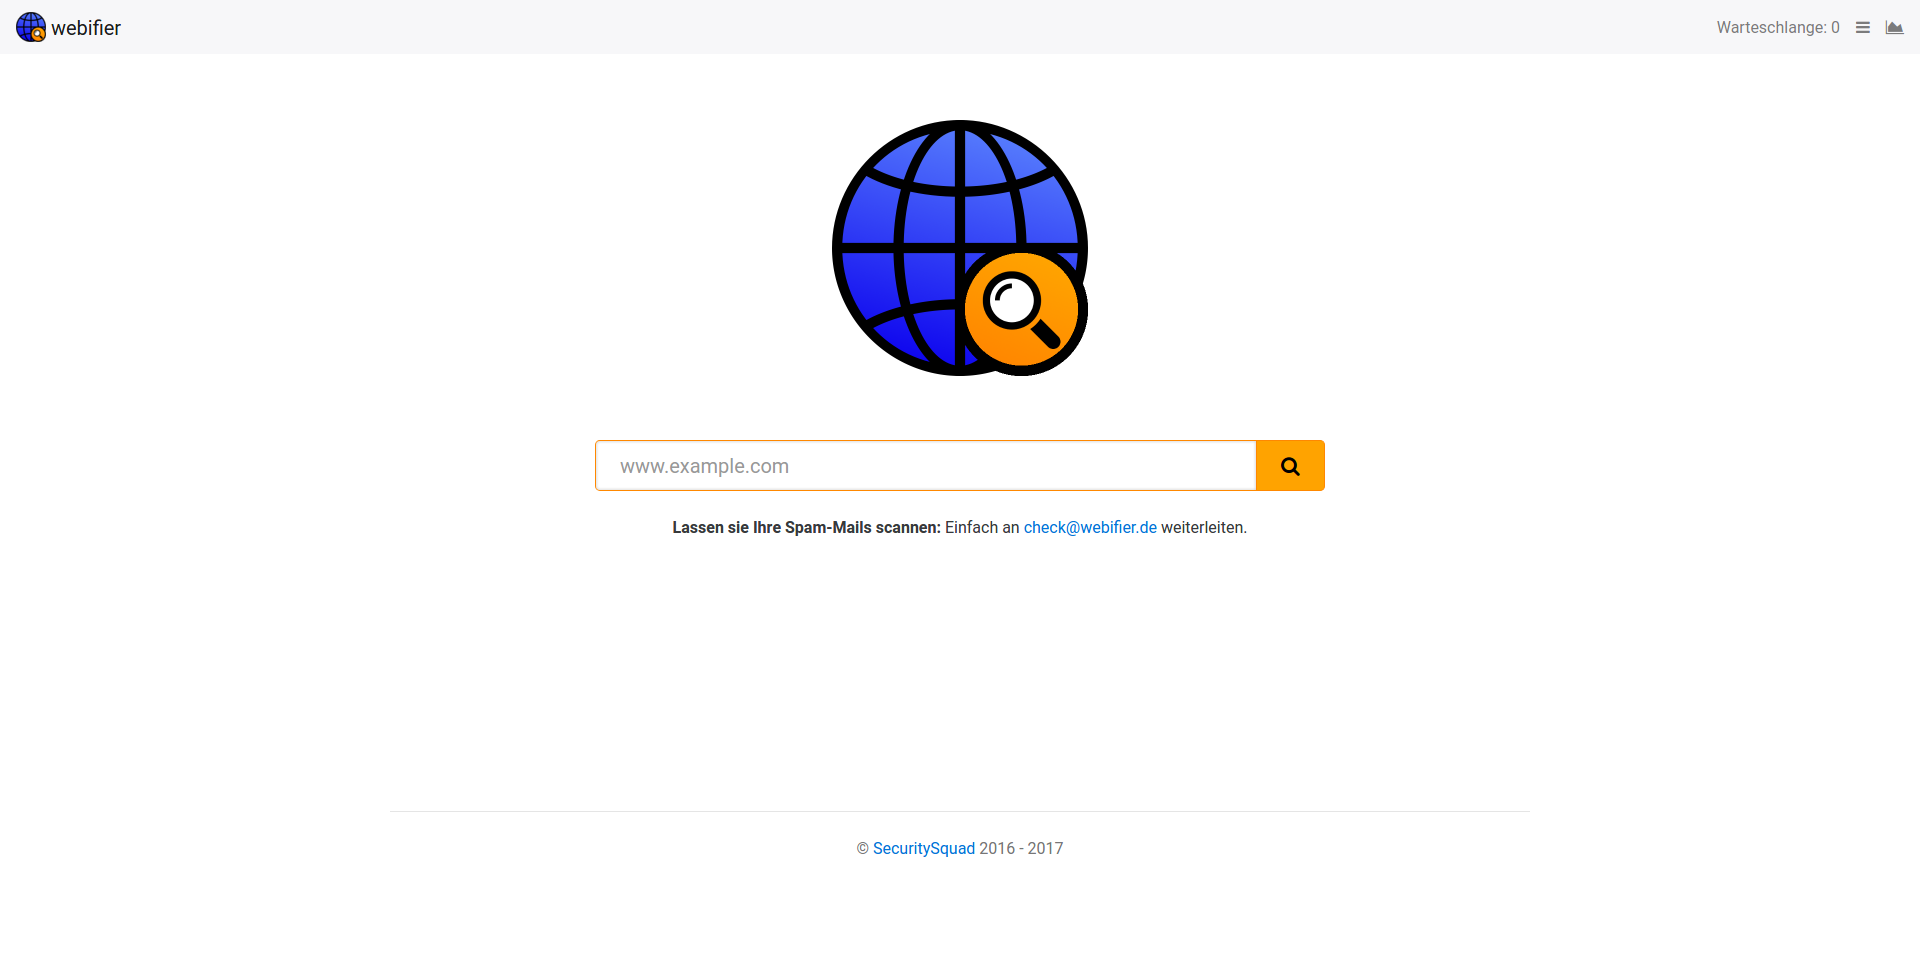
\includegraphics[width=\textwidth]{images/platform/screenshot-start}
  \caption[webifier Platform - Startseite]{webifier Platform - Startseite\protect\footnotemark}
  \label{fig:platform-start}
\end{figure}
\footnotetext{Die Abbildung befindet sich in besserer Qualität in Anhang \appref{d}.}

Nachdem die Überprüfung einer Webseite gestartet wurde wird der Nutzer auf die in Abbildung \ref{fig:platform-result} abgebildete Seite geleitet, welche sich nach und nach mit den Ergebnissen der einzelnen Tests füllt, sobald diese vorliegen. Sind alle Tests beendet, wird auch das Endresultat angezeigt. Die Ergebnisseite bietet zunächst einen kompakten Überblick über alle ausgeführten Tests und deren Ergebnisse.

\begin{figure}[H]
  \centering
  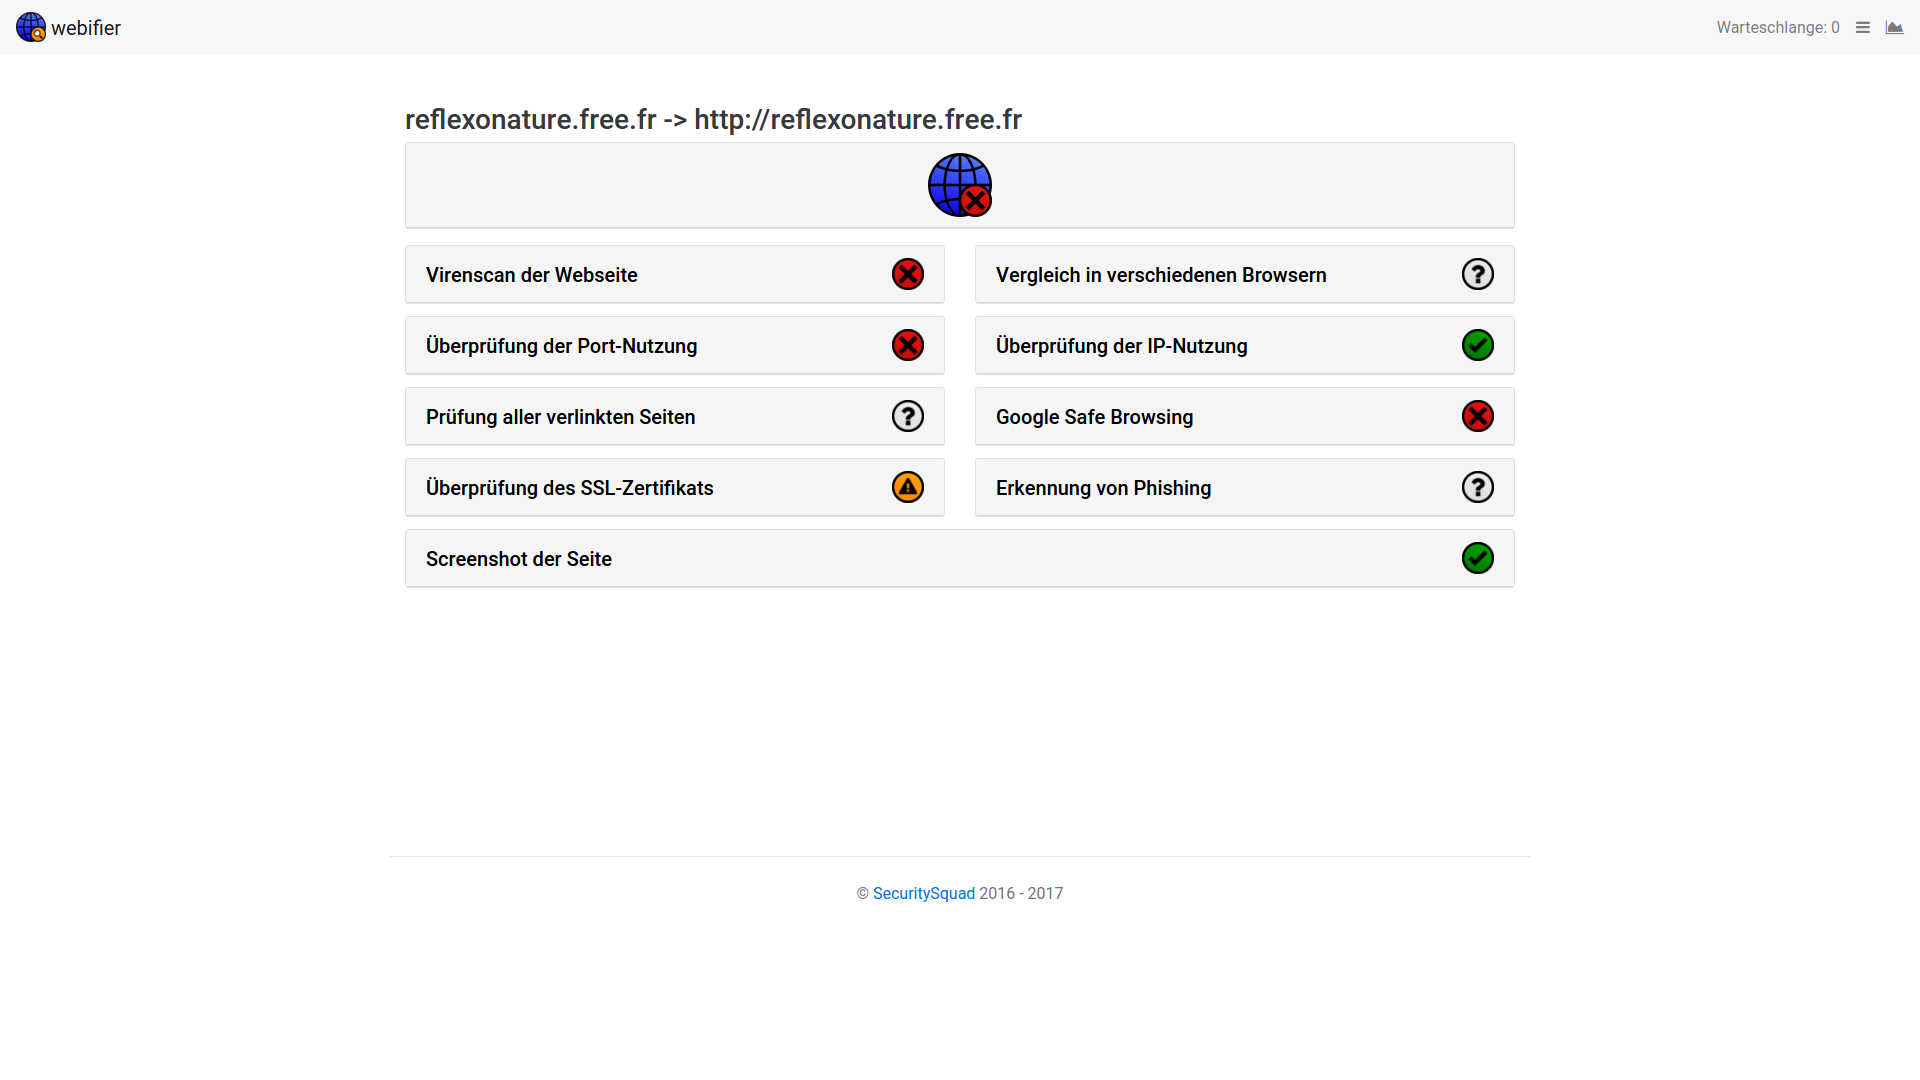
\includegraphics[width=\textwidth]{images/platform/screenshot-reflexonature}
  \caption[webifier Platform - Ergebnisseite]{webifier Platform - Ergebnisseite\protect\footnotemark}
  \label{fig:platform-result}
\end{figure}
\footnotetext{Diese und weitere Ergebnisseiten befinden sich in besserer Qualität in Anhang \appref{d}.}

Möchte der Nutzer noch genauere Informationen zu den Ergebnissen eines Tests, so lassen sich alle Testfelder mit einem Klick darauf ausklappen. Im Folgenden werden nun die Detailansichten der einzelnen Testergebnisse gezeigt und erläutert.

\begin{figure}[H]
  \centering
  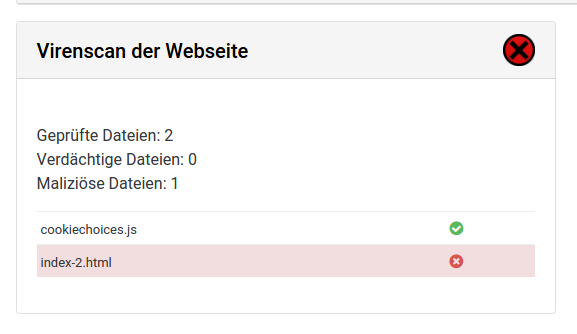
\includegraphics[width=7.5cm]{images/platform/virusscan-malicious}
  \caption{webifier Platform - Virenscan der Webseite}
  \label{fig:platform-result-virusscan}
\end{figure}

Die Detailansicht des Virenscans, welche in Abbildung \ref{fig:platform-result-virusscan} dargestellt ist, zeigt einmal die Anzahl aller gescannten Dateien, sowie die Anzahlen der gefundenen verdächtigen oder maliziösen Dateien. Außerdem erhält die Ansicht eine genaue Auflistung aller Dateien mit entsprechendem Ergebnis. So lässt sich genau feststellen, welche Dateien welche Bedrohung darstellen.

\begin{figure}[H]
\centerline{%
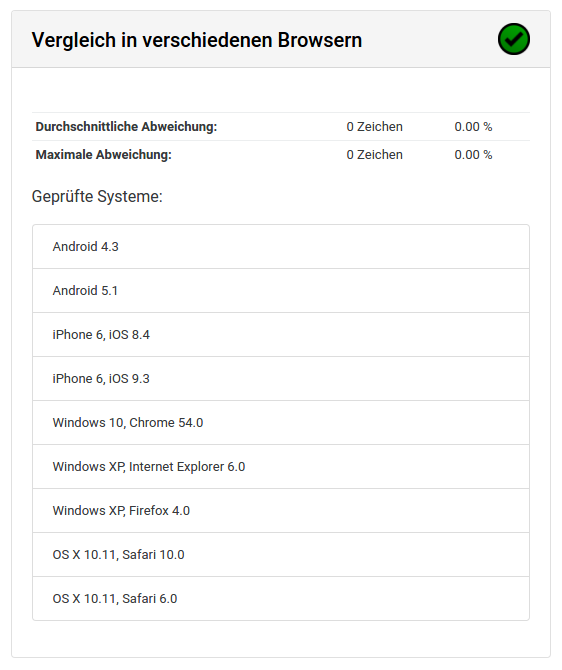
\includegraphics[width=0.5\textwidth]{images/platform/header-inspection-clean}%
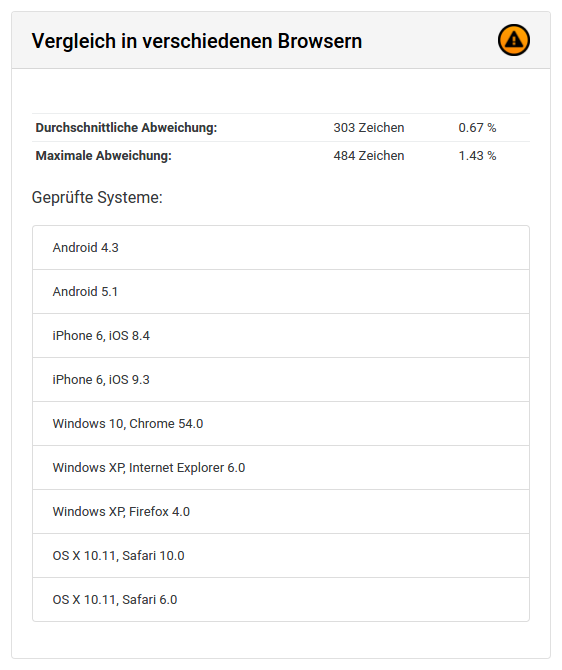
\includegraphics[width=0.5\textwidth]{images/platform/header-inspection-suspicious}%
}%
\caption{webifier Platform - Vergleich in verschiedenen Browsern}
\label{fig:platform-result-header-inspection}
\end{figure}

Der Vergleich in verschiedenen Browsern zeigt die maximale und die durchschnittliche Abweichung, sowohl als absoluten, als auch als prozentualen Wert. Zusätzlich erhält der Nutzer eine Übersicht uber alle Systeme, welche getestet und miteinander verglichen wurden. Zwei Beispielergebnisse hierfür sind in Abbildung \ref{fig:platform-result-header-inspection} zu sehen.

\begin{figure}[H]
\centerline{%
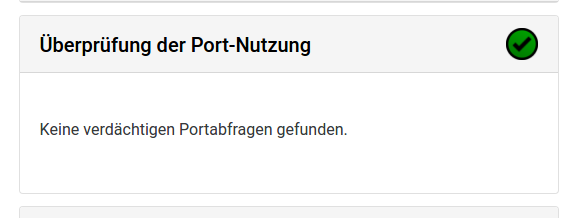
\includegraphics[width=0.5\textwidth]{images/platform/portscan-clean}%
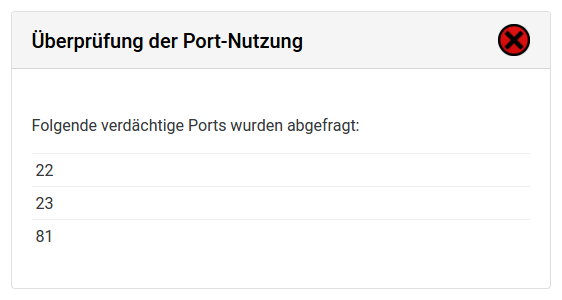
\includegraphics[width=0.5\textwidth]{images/platform/portscan-malicious}%
}%
\caption{webifier Platform - Überprüfung der Port-Nutzung}
\label{fig:platform-result-portscan}
\end{figure}

\begin{figure}[H]
  \centering
  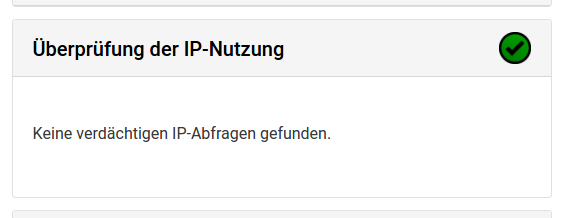
\includegraphics[width=7.5cm]{images/platform/ipscan-clean}
  \caption{webifier Platform - Überprüfung der IP-Nutzung}
  \label{fig:platform-result-ipscan}
\end{figure}

Abbildung \ref{fig:platform-result-portscan} zeigt die Ergebnisse der Überprüfung der Port-Nutzung, welche im Falle eines verdächtigen oder bedrohlichen Ergebnisses eine Liste mit allen gefundenen Ports enthält. Das Ergebnis der Überprüfung der IP-Nutzung ist gleich aufgebaut und in Abbildung \ref{fig:platform-result-ipscan} abgebildet. Es stellt bei entsprechenden Funden eine Liste aller IP-Adressen bereit.

\begin{figure}[H]
  \centering
  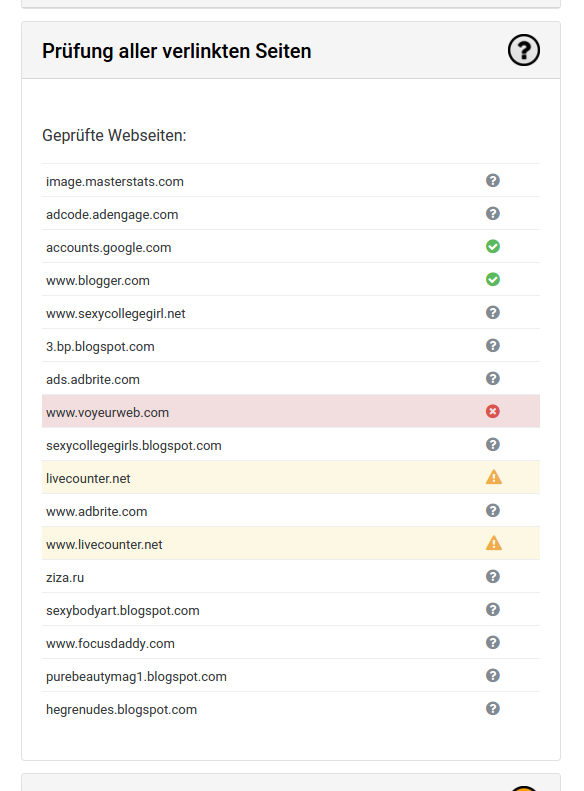
\includegraphics[width=7.5cm]{images/platform/linkchecker-undefined}
  \caption{webifier Platform - Prüfung aller verlinkten Seiten}
  \label{fig:platform-result-linkchecker}
\end{figure}

Das Ergebnis der Prüfung aller verlinkten Seiten enthält eine einfache Liste mit allen gefundenen Links und dem entsprechenden Ergebnis aus webifier Data. Abbildung \ref{fig:platform-result-linkchecker} zeigt eine solche Liste.

\begin{figure}[H]
\centerline{%
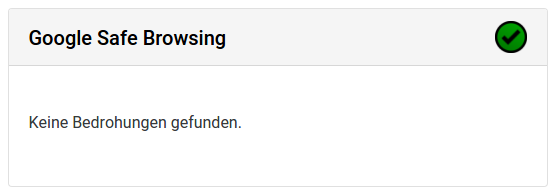
\includegraphics[width=0.5\textwidth]{images/platform/google-safe-browsing-clean}%
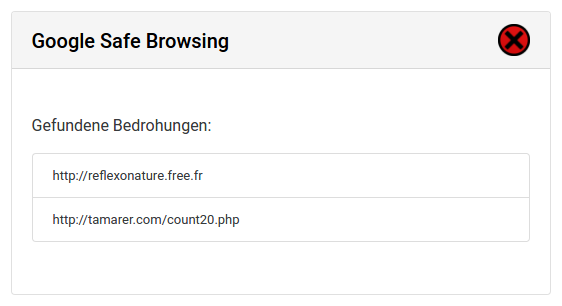
\includegraphics[width=0.5\textwidth]{images/platform/google-safe-browsing-malicious}%
}%
\caption{webifier Platform - Google Safe Browsing}
\label{fig:platform-result-google-safe-browsing}
\end{figure}

Die Deteilansicht des Google Safe Browsing Ergebnisses ist ähnlich dem der Prüfung aller verlinkten Seiten. Allerdings listet diese nur alle gefundenen Bedrohungen auf und nicht alle geprüften Links. Abbildung \ref{fig:platform-result-google-safe-browsing} enthält zwei Beispielresultate.

\begin{figure}[H]
\centerline{%
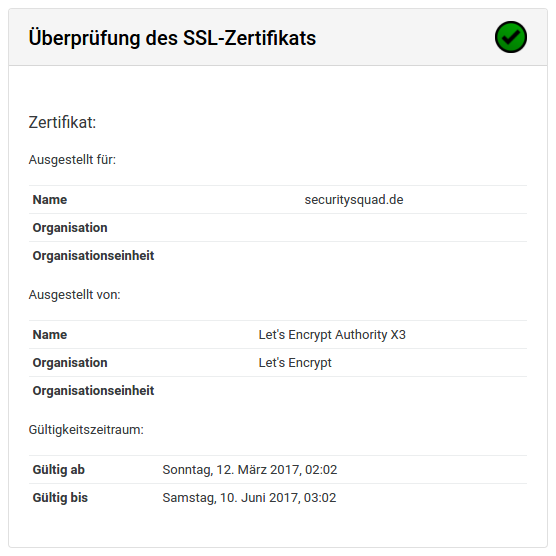
\includegraphics[width=0.5\textwidth]{images/platform/certificatechecker-clean}%
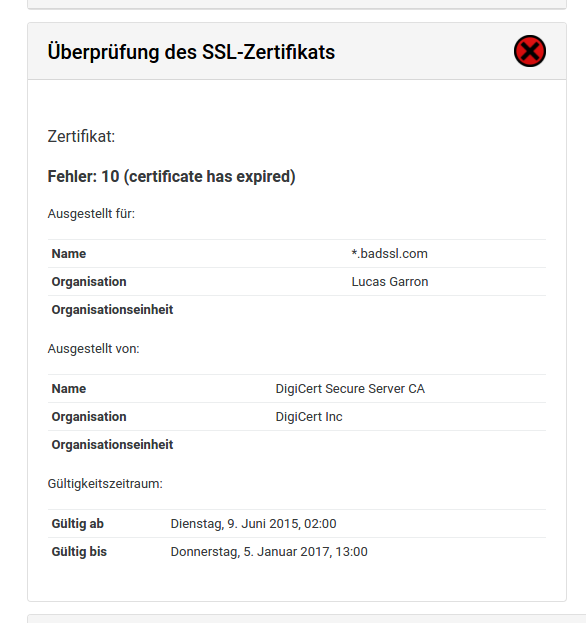
\includegraphics[width=0.5\textwidth]{images/platform/certificatechecker-malicious}%
}%
\caption{webifier Platform - Überprüfung des SSL-Zertifikats}
\label{fig:platform-result-certificatechecker}
\end{figure}

Das Ergebnis der Überprüfung des SSL-Zertifikates enthält alle Informationen des Zertifikats, sofern die Webseite eines nutzt. Wie in Abbildung \ref{fig:platform-result-certificatechecker} dargestellt, zeigt die Detailansicht einmal für wen das Zertifikat ausgestellt wurde, aber auch wer es ausgestellt hat. Außerdem wird der Gültigkeitszeitraum des Zertifikats angezeigt und im Fehlerfall der gefundene Fehler.

\begin{figure}[H]
\centerline{%
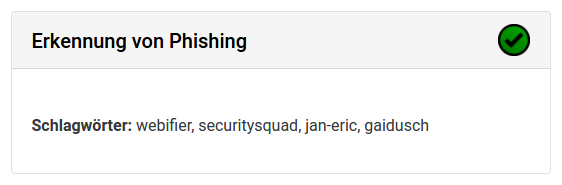
\includegraphics[width=0.5\textwidth]{images/platform/phishing-clean}%
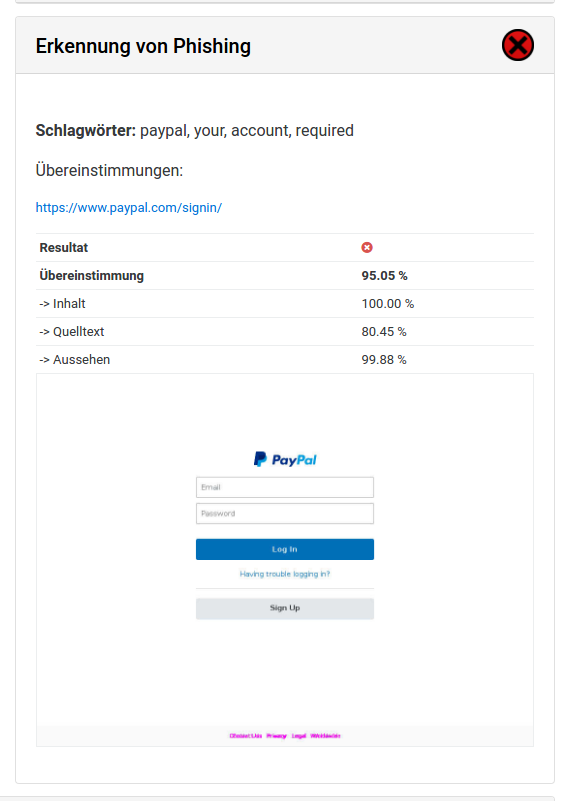
\includegraphics[width=0.5\textwidth]{images/platform/phishing-malicious}%
}%
\caption{webifier Platform - Erkennung von Phishing}
\label{fig:platform-result-phishingdetector}
\end{figure}

Die Erkennung von Phishing stellt ebenfalls einige Informationen zur Verfügung, wie Abbildung \ref{fig:platform-result-phishingdetector} zeigt. Es werden in jedem Fall die gefundenen Schlagwörter der Webseite angezeigt. Ist das Ergebnis verdächtig oder bedrohlich, so wird die vermeindliche Originalseite verlinkt, die Werte der prozentualen Übereinstimmungen insgesamt und von Inhalt, Quelltext und Aussehen separat aufgelistst und ein Bild der beiden überlagerten Seiten gezeigt. Alle Inhalte, welche sich unterscheiden werden rosa dargestellt. Im Beispiel aus der Abbildung unterscheidet sich demnach nur der Text der Fußzeile.

\begin{figure}[H]
  \centering
  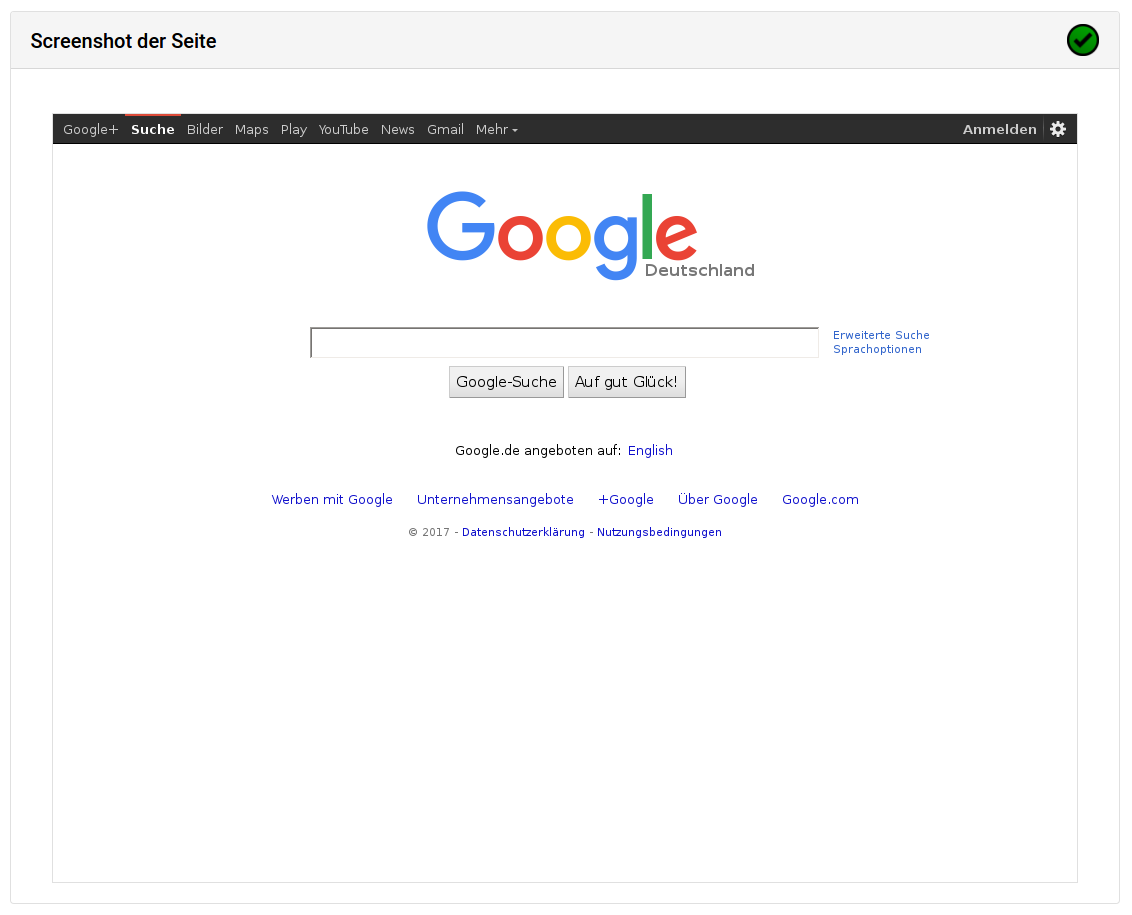
\includegraphics[width=\textwidth]{images/platform/screenshot-clean}
  \caption{webifier Platform - Screenshot der Seite}
  \label{fig:platform-result-screenshot}
\end{figure}

Der Screnenshot der Seite wird beim ausklappen des Panels einfach angezeigt, so wie es in Abbildung \ref{fig:platform-result-screenshot} dargestellt. Dies gibt dem Nutzer die Möglichkeit sich die Webseite anzusehen, ohne sie selbst zu besuchen.

Wie nun gezeigt bietet die Plattform seh viele interessante Zusatzinformationen zu den Testergebnissen, mit denen das Gesamtresultat noch genauer erklärt wird. Außerdem bekommt der Nutzer so genügend Informationen um die Plausibilität der Testergebnisse selbst noch einmal zu überprüfen.

\subsection{webifier Mail}

\todo{Daniel}

\subsection{webifier Data}
\label{sec:umsetzung-data}

webifier Data stellt eine Schnittstelle zur globalen Datenspeicherung der Testresultate zur Verfügung. Die Komponente setzt ebenfalls auf dem Spring-Framework auf und wurde deshalb in Java implementiert. Außerdem wird die Spring-Bibliothek Spring-Data eingesetzt um Java-Objekte auf Dokumente zu übertragen und in einer MongoDB zu persistieren.

Das Modul bietet eine \ac{REST}-\ac{API} zur externen Nutzung, beispielsweise im webifier Tester oder in der Prüfung aller verlinkten Seiten. Die API stellt die folgenden Aktionen bereit: \lstinline[style=eclipse]{/push}, \lstinline[style=eclipse]{/check} und \lstinline[style=eclipse]{/count}. Mit der Methode \lstinline[style=eclipse]{/push} können Testergebnisse in webifier Data abgelegt werden. Die entsprechende Resource, welche im Inhalt des POST-Requests gesendet werden muss ist in Listing \ref{lst:data-push} dargestellt.

\begin{scriptsize}
\lstset{
    style=eclipsejavascript,
    caption={Ausschnitt Inhalt push-Request - webifier Data},
    label={lst:data-push}
}
\begin{lstlisting}
{
    "id" : "33e76954-dc94-48a9-a816-99ddeb647887",
    "enteredUrl" : "securitysquad.de",
    "testedUrl" : "https://www.securitysquad.de/",
    "result" : {
        "resultType" : "CLEAN",
        "resultValue" : 0
    }
    "duration" : 46220,
    "testResults" : [
        {
            "testId" : "33e76954-dc94-48a9-a816-99ddeb647887_07bb1b72-fd9f-4286-ade5-2d71cf47580a",
            "testData" : {
                "name" : "VirusScan",
                "startup" : "docker run --rm --name #ID -e URL=#URL -e ID=#ID webifier-test-virusscan",
                "shutdown" : "docker stop #ID",
                "enabled" : true,
                "weight" : 5,
                "startupTimeoutInSeconds" : 600,
                "shutdownTimeoutInSeconds" : 30,
            },
            "result" : {
                "result" : "CLEAN",
                "resultInfo" : {
                    ...
                }
            },
            "duration" : 31191
        },
        ...
    ]
}
\end{lstlisting}
\end{scriptsize}

Die Methode \lstinline[style=eclipse]{/check} bietet die Möglichkeit webifier Data nach einer oder mehreren Urls zu durchsuchen. Hierfür muss im Inhalt des POST-Requests die in Listing \ref{lst:data-check-request} gezeigte Ressource gesendet werden. Diese enthält eine Liste der zu überprüfenden Links.

\begin{scriptsize}
\lstset{
    style=eclipsejavascript,
    caption={Inhalt check-Request - webifier Data},
    label={lst:data-check-request}
}
\begin{lstlisting}
{
    "urls": [
        "https://fonts.googleapis.com/css?family=Montserrat:400,700",
        "https://fonts.googleapis.com/css?family=Lato:400,700,400italic,700italic",
        "https://www.google.com/recaptcha/api.js",
        "https://cdnjs.cloudflare.com/ajax/libs/jquery-easing/1.3/jquery.easing.min.js",
        "https://www.gstatic.com/recaptcha/api2/r20170503135251/recaptcha__de.js",
        "https://fonts.gstatic.com/s/lato/v13/v0SdcGFAl2aezM9Vq_aFTQ.ttf",
        "https://fonts.gstatic.com/s/lato/v13/DvlFBScY1r-FMtZSYIYoYw.ttf",
        "https://www.gstatic.com/recaptcha/api2/r20170503135251/fallback__ltr.css",
        "https://fonts.googleapis.com/css?family=Roboto:400,500",
        "https://www.gstatic.com/recaptcha/api2/logo_48.png",
        "https://github.com/SecuritySquad",
        "https://www.webifier.de/",
        "https://github.com/SecuritySquad/webifier-platform",
        "http://djbrown.de/",
        "https://www.facebook.com/danjoebro",
        "https://github.com/djbrown",
        "https://plus.google.com/114056971447496286521",
        "https://github.com/jockelmore",
        "https://samuel-philipp.de/",
        "https://github.com/samuel-p",
        "https://plus.google.com/u/0/+SamuelPd"
    ]
}
\end{lstlisting}
\end{scriptsize}

Wie Listing \ref{lst:data-check} zeigt gruppiert webifier Data zunächst alle Links anhand deren Host-Teil und entfernt alle ungültigen Einträge. Anschließend werden alle Resultate für jeden Eintrag der Liste geladen und daraus ein Gesamtergebnis pro Host berechnet. Dieses wird schließlich mit dem Host als schlüssel zur Liste \textit{hostResults} hinzugefügt. Abschließend wird die erzeugte Liste als Ergebnis zurückgegeben und als Antwort zurückgesendet. Diese Antwort ist in Listing \ref{lst:data-check-response} abgebildet.

\begin{scriptsize}
\lstset{
    style=eclipsejava,
    caption={Verarbeitung check Methode - webifier Data},
    label={lst:data-check}
}
\begin{lstlisting}
$$@Override$$
public WebifierCheckTestResultsResponse checkTestResultsRequest(WebifierCheckTestResultsRequest request) {
    List<String> hosts = request.getUrls().stream().map(url -> {
        try {
            return filterHost(url);
        } catch (MalformedURLException e) {
            return null;
        }
    }).distinct().filter(StringUtils::isNotEmpty).collect(toList());
    Map<String, WebifierTestResultDetails> hostResults = new HashMap<>();
    hosts.forEach(host -> {
        List<WebifierTestResultData> data = #dataPersistenceService#.getTestResultDataByHost(host)
                .stream().filter(d -> d.getOverallResultType() != WebifierTestResult.##UNDEFINED##).collect(toList());
        if (data.isEmpty()) {
            hostResults.put(host, WebifierTestResultDetails.##UNDEFINED##);
        } else {
            double resultValue = data.stream().mapToDouble(this::mapDataResultToIndex).average().orElse(1);
            hostResults.put(host, mapResultValueToResult(resultValue));
        }
    });
    if (hostResults.isEmpty()) {
        return new WebifierCheckTestResultsResponse(false);
    }
    return new WebifierCheckTestResultsResponse(true, hostResults);
}
\end{lstlisting}
\end{scriptsize}

\begin{scriptsize}
\lstset{
    style=eclipsejavascript,
    caption={Inhalt check-Response - webifier Data},
    label={lst:data-check-response}
}
\begin{lstlisting}
{
    "success": true,
    "hosts": {
        "www.facebook.com": "CLEAN",
        "fonts.googleapis.com": "UNDEFINED",
        "plus.google.com": "CLEAN",
        "fonts.gstatic.com": "UNDEFINED",
        "cdnjs.cloudflare.com": "UNDEFINED",
        "github.com": "CLEAN",
        "djbrown.de": "UNDEFINED",
        "samuel-philipp.de": "UNDEFINED",
        "www.google.com": "SUSPICIOUS",
        "www.gstatic.com": "UNDEFINED",
        "www.webifier.de": "CLEAN"
    }
}
\end{lstlisting}
\end{scriptsize}

Die Methode \lstinline[style=eclipse]{/count} liefert einfach die aktuelle Gesamtzahl der in webifier Data vorhandenen Testergebnisse.

Die Testergebnisse werden in der MongoDB auf zwei Dokumente verteilt. Das erste Dokument (\lstinline[style=eclipse]{webifierTestResultData}) enthält alle Gesamtdaten des Resultats, das zweite (\lstinline[style=eclipse]{webifierSingleTestResultData}) umfasst alle Einzelergebnisse des Resultats. Deshalb werden pro Testergebnis ein Dokument in \lstinline[style=eclipse]{webifierTestResultData} und acht in \lstinline[style=eclipse]{webifierSingleTestResultData} gespeichert.

Zur Persistierung werden alle Informationen der \lstinline[style=eclipse]{/push} Methode (Listing \ref{lst:data-push}) auf die entspechenden Dokumente gemappt. Listing \ref{lst:data-resultdata} zeigt die transformierten Daten aus \lstinline[style=eclipse]{webifierTestResultData}. Anhang \appref{e} enthält die transformierten Dokumente aller Einzelergebnisse in \lstinline[style=eclipse]{webifierSingleTestResultData}.

\begin{scriptsize}
\lstset{
    style=eclipsejavascript,
    caption={Beispieldokument webifierTestResultData - webifier Data},
    label={lst:data-resultdata}
}
\begin{lstlisting}
{
	"_id" : "d62e8c94-21c9-4d69-9337-186b38f73cce",
	"_class" : "de.securitysquad.webifier.persistence.domain.WebifierTestResultData",
	"testerId" : "56821bd8-f652-4b59-b7ec-12faa7cf6cae",
	"enteredUrl" : "ukauctionline.co.uk",
	"testedUrl" : "http://ukauctionline.co.uk",
	"host" : "ukauctionline.co.uk",
	"overallResultType" : "SUSPICIOUS",
	"overallResultValue" : 0.057291666666666664,
	"durationInMillis" : NumberLong(227639),
	"datetime" : ISODate("2017-03-28T22:32:53.834Z"),
	"testResults" : [
		DBRef("webifierSingleTestResultData", "5ecb25e6-457b-41ab-9241-a60f8a484131"),
		DBRef("webifierSingleTestResultData", "abb70569-64d3-47ae-b3e3-ff8086c8f937"),
		DBRef("webifierSingleTestResultData", "56dbbcb3-9628-4dd4-bb20-692bd86c5410"),
		DBRef("webifierSingleTestResultData", "64ae09d4-a79e-4194-b77c-3a7891342567"),
		DBRef("webifierSingleTestResultData", "05ba8488-4b69-40f9-8a9d-661c09daab65"),
		DBRef("webifierSingleTestResultData", "e0ce8955-feb7-4f7a-adfb-b7b8116a9d28"),
		DBRef("webifierSingleTestResultData", "9affd5e9-37eb-4d83-b471-ceab0c19155c"),
		DBRef("webifierSingleTestResultData", "c2b02bf9-2073-451b-a566-295fe1801e51")
	]
}
\end{lstlisting}
\end{scriptsize}

\subsection{webifier Statistics}
\label{sec:umsetzung-statistics}

Webifier Statistics wird in R implementiert. Hierzu werden Flexdashboards\footnote{\url{http://rmarkdown.rstudio.com/flexdashboard/index.html}} verwendet. Zur Generierung der Grafiken wurde auf verschiedene Librarys, wie beispielsweise Plot.ly, zurückgegriffen um den Entwicklungsaufwand für die Visualisierungen zu minimieren. Die Anordnung der Grafiken wird über ein bestimmtes Layout definiert. Jede Grafik wird prinzipiell in 3 Schritten erstellt:

\begin{enumerate}
  \item Daten aus der MongoDB laden
  \item Daten in die benötigte Form transformieren
  \item Entsprechende API ansteuern für Generierung der Grafik
\end{enumerate}

\begin{scriptsize}
\lstset{
    style=eclipsejavascript,
    caption={Beispiel R-Grafik},
    label={lst:rgrafik}
}
\begin{lstlisting}
  ### Durchschnittliche Analysezeit

  ```{r}
  result <- dbGetQueryForKeys(mg1, 'webifierTestResultData',"{}", "{durationInMillis:1}",skip=0,limit=Inf)
  mean.dur <- mean(result$durationInMillis)/1000
  mean.dur <- round(mean.dur)
  tp <- seconds_to_period(mean.dur)
  valueBox(paste(minute(tp),'min ',second(tp),'s',sep=""), icon="fa-hourglass-half",color="grey")
  ```
\end{lstlisting}
\end{scriptsize}

Im Codebeispiel \ref{lst:rgrafik} ist der Codeablauf für eine Valuebox zu sehen. Dieses Beispiel wurde ausgewählt um den Erstellungsprozess für die Grafiken zu erklären. Dies lässt sich auf alle anderen Grafiken übertragen.

Die Überschriften der Grafiken werden mit \textit{\#\#\#} markiert. Der R-Code befindet sich in Chunks, diese werden speziell markiert um dem Compiler kenntlich zu machen welches der R-Code ist.

Im Beispiel werden zunächst benötigten Daten aus der MongoDB geladen. Da hier eine Valuebox für die Anzeige der durchschnittlichen Analysezeit generiert wird werden nur die Analysezeiten(durationInMillis) benötigt. Diese werden anschließend gemittelt und von Millisekunden in Minuten/Sekunden transformiert. Zur Erstellung der Valuebox muss nun nurnoch der Text, die Farbe und ein passendes Icon ausgewählt werden. Die Generierung und Platzierung übernimmt Flexdashboard. Als Ausgabe wird eine HTML-Datei generiert, welche dann in den Webserver eingebunden wird um sie für die Nutzer zugänglich zu machen.

\begin{figure}[H]
  \centering
  
\includegraphics[width=5cm]{images/stats/valuebox}
  \caption{Generierte Valuebox}
  \label{fig:valuebox}
\end{figure}

In Abbildung \ref{fig:valuebox} ist die fertig generierte Valuebox mit Überschrift, Text und Icon in passender Farbe dargestellt.

Für stets aktuelle Grafiken wird das R-Skript für die Statistiken mehrfach täglich neu gebaut um die aktuellen Daten mit einzubeziehen. Von einer \textit{On the fly}-Generierung der Grafiken wurde abgesehen, da dies für den Server zu rechenintensiv wäre.

\section{Tests}

In diesem Abschnitt werden nun die Implementierungen aller Einzeltests erklärt. Bei allen kam zur Isolierung die Technologier Docker zum Einsatz.

\subsection{Virenscan der Webseite}

Der Virenscan der Webseite wurde in Python umgesetzt und lädt zunächst alle Ressourcen der Webseite in ein lokales Verzeichnis herunter. Hierbei kommt die Software HTTrack zum Einsatz. HTTtrack wird für diesen Zweck speziell konfiguriert, um die Antwortzeiten so gering wie möglich zu halten. Zunächst wird der Downloadmodus so gewählt, dass einfach nur alle Dateien gespeichert werden, ohne sie für die dauerhafte Nutzung bereitzuhalten. Des weiteren darf keine Datei im Inhalt verändert werden, da so das Ergebnis verfälscht werden könnte. Um zeit zu spaaren wird zusätzlich auf die protokollierung verzichtet. Außerdem sollen die \lstinline[style=eclipse]{robots.txt} Dateien ignoriert werden, da damit Malware auch vor Suchmaschinen versteckt werden kann. Schießlich wird HTTrack eine maximale Laufzeit zum Download aller Dateien von drei Minuten gewährt.

Zum Scannen aller gespeicherten Dateien kommen drei Virenscanner zum Einsatz. Es werden die Antivirenprogramme ClamAV\footnote{\url{http://www.clamav.net/}}, AVG\footnote{\url{http://www.avg.com/de-de/homepage}} und Comodo Antivirus\footnote{\url{https://antivirus.comodo.com/}} verwendet. Um auch hier die Antwortzeiten gering zu halten werden die Virenscannner parallel ausgeführt.

Abschließend werden alle Ergebnisse der Antivirenprogramme ausgewertet und daraus das Gesamtergebnis gebildet. Dieses wird inklusive der Liste aller bewertetetn Dateien weitergeleitet.

\subsection{Vergleich in verschiedenen Browsern}

Dieser Test wird durch zwei Schritte ermöglicht.
Zunächst werden für eine Liste von Browserkonfigurationen deren \ac{HTTP}-Header ermittelt, danach werden Requests mit diesen Headern an die zu testende \ac{URL} geschickt und die Antworten untereinander verglichen.
Damit nicht bei jedem Testdurchlauf alle Header neu eingeholt werden müssen, werden sie in einer Datei abgespeichert.

Zur Umsetzung dieses Tests wurde zunächst das Python-Skript \lstinline{collect.py} geschrieben, welches über einen Cloud-Service die Werte für das \ac{HTTP}-Headerfeld \textit{User Agent} abspeichert.
Zuerst werden alle gewünschten Browserkonfigurationen über eine \ac{JSON}-Datei eingelesen (s. Zeile 31).
Diese Datei enthält eine Liste von Browserobjekten, die die Konfigurationen im Attribut 
Ein Element dieser Liste ist beispielhaft in \autoref{lst:browsers.json} zu sehen, wobei das \lstinline{"headers"}-Attribut vor Programmablauf noch nicht gesetzt ist.

\begin{scriptsize}
\lstset{
	style=eclipsejavascript,
	caption={Beispiel für Browserkonfiguration und gespeicherte Header},
	label={lst:browsers.json}
}
\begin{lstlisting}
[{"configuration": {
    "platform": "Windows XP",
    "browserName": "internet explorer",
    "version": "6.0",
    "name": "Windows XP, Internet Explorer 6.0"
  },
  "headers": {
    "Host": "www.reliply.org",
    "Request Method": "GET",
    "User Agent": "Mozilla/4.0 (compatible; MSIE 6.0; Windows NT 5.2; SV1; .NET CLR 1.1.432)",
    "Accept Encoding": "gzip, deflate",
    "Accept Language": "en-us",
    "HTTP Connection": "keep-alive"
}}]
\end{lstlisting}
\end{scriptsize}

Danach werden für jeder dieser Konfigurationen die entsprechenden Header ermittelt.
Dazu wird eine Verbindung mittels \ac{SSH} zum Service \textit{Sauce Labs} aufgebaut.
Dabei wird auch ein ferngesteuerter Browser mit der Konfiguration des lokalen Browserobjekts initialisiert.
Das Browserobjekt ist wie ein Headless Browser über das Modul \textit{WebDriver} steuerbar.
Im nächsten Schritt wird der Browser dann angewiesen auf die Webseite \url{http://www.reliply.org/tools/requestheaders.php} zu gehen.
Auf dieser Seite werden alle \ac{HTTP}-Headerfelder und deren Werte in einer Tabelle aufgelistet.
Ein Beispiel dafür ist in \autoref{fig:reliply} zu sehen.
Diese Tabelle beinhaltet in der ersten Spalte den Headernamen und in der zweiten den Wert.
Diese beiden Daten werden in jeder Zeile der Tabelle 
Der Brower greift auf diese beiden Daten in jeder Zeile der Tabelle zu und speichert diese im Browserobjekt.
Es werden alle Header bis auf den \lstinline{Host}-Header abgespeichert, da dieser lediglich der Domain des Zielserver entspricht.
Nachdem alle Header zu den Browserkonfigurationen heruntergeladen wurden, wird die Liste der Browserobjekte in die Datei \lstinline{browser.json} abgespeichert.

\begin{figure}[H]
	\centering
	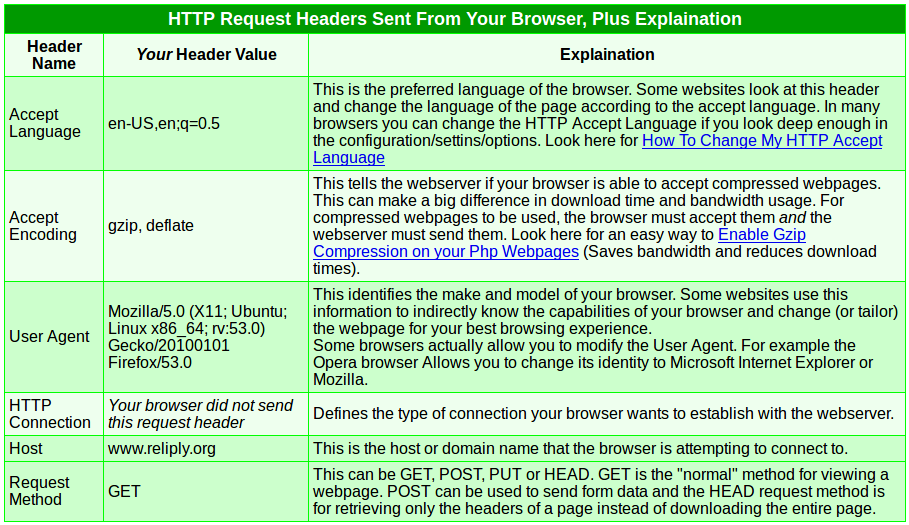
\includegraphics[width=\textwidth]{images/reliply.png}
	\caption{Tabelle der \ac{HTTP}-Header auf \url{reliply.org}}
	\label{fig:reliply}
\end{figure}

Bei der Testausführung wird dann das Python-Skript \lstinline{check.py} aufgerufen.
Darin wird zunächst die Liste der Browserobjekte aus der Datei geladen.
Danach wird über das Packet \textit{requests} für jeden Browser ein \ac{HTTP}-Request an die zu testende Seite geschickt.
Die Antwort wird wiederum im Browserlement gespeichert, sodass es für die folgenden Vergleiche zur Verfügung steht.

Es werden alle Browser jeweils genau einmal mit allen anderen Browsern verglichen.
Das bedeutet, dass das erste Element mit allen weiteren $n-1$ Elementen verglichen werden muss. Das zweite mit den letzten $n-2$ usw.
Das Vorletzte muss dann nur noch mit dem letzten Element verglichen werden, was vom informatischen Aufwand her abschätzbar ist durch den Aufwand der Gau"sschen Summenformel ($\frac{n^2+n}{2}$).
Dieser Algorithmus hat also eine Komplexität von $\mathcal{O}(n^2)$ und kann damit zum Engpass werden, falls es zu viele Browser geben sollte.

Ursprünglich basierte die Berechnung der Abweichungen auf Prozentwerten.
Während der Implementierung ist aufgefallen, dass die prozentualen Abweichungen der Antworten keine zuverlässige Auskunft über einen möglichen Angriff auf den Nutzer geben können.
Aus diesem Grund wird die Ergebniskalkulation nun auf absoluten Abweichungswerten ausgeführt.
Jede Browserantwort wird jeweils einmal mit jeder anderen verglichen und der niedrigste absolute Übereinstimmungswert als \lstinline{worst\_diff} gespeichert.
Es wird der schlechteste Übereinstimmungswert für die Ergebnisberechnung gewählt, da er bei einer Durchschnitts- oder Medianberechnung  statistisch untergehen würde und somit gezielte Angriffe gegen eine Browsergruppe nicht regstriert werden würden.
Zur Berechnung dieses Wertes werden zunächst die übereinstimmenden Blöcke der beiden Antworten durch das \textit{statistics}-Paket von Python ermittelt.
Durch diese wird die gesamte Übereinstimmungslänge berechnet, die dann von der Gesamtlänge der größeren Antwort abgezogen wird.
Zur Ergebnisberechnung wird schließlich überprüft, ob der schlechteste Wert unter einer bestimmten Grenze liegt.
Liegt der Wert über 500, dann ist das Ergebnis \textit{MALICIOUS}.
Liegt der Wert zwischen 500 und 50, so ist das Ergebnis \textit{SUSPICIOUS}, ansonsten ist es \textit{CLEAN}.

\subsection{Überprüfung der Port-Nutzung}
Bei diesem Test wird überprüft ob die Seite versucht einen Portscan auf dem Computer des Anwenders zu betreiben. Hierfür werden 3 Techniken eingesetzt. Die wichtigsten Aufgaben werden von PhantomJS und Bro erledigt.
Bro ist ein Netzwerkmonitoringtool und wird hier genutzt um den Traffic welcher zwischen Webseite und Client entsteht zu protokollieren und in einer Logdatei abzuspeichern. PhantomJS ist ein \textit{headless Browser}, welcher genutzt wird um die Webseite aufzurufen und dessen Javascript auszuführen. Das ganze funktioniert hier ohne grafische Oberfläche.

Der Ablauf des Tests sieht wie folgt aus: Zunächst wird Bro intialisiert und es werden Filter angelegt um lediglich die Ports, der eingehenden Anfragen, mitzuloggen und in der Logdatei abzuspeichern. Ist Bro vollständig initialisiert und einsatzbereit startet PhantomJS mit dem Aufrufen der Seite und Ausführen des JavaScript-Codes. Währenddessen speichert Bro alle Netzwerkaktivitäten. Sobald der Durchlauf von PhantomJS abgeschlossen ist wird mittels Python die Validierung des Ergebnisses gestartet. Hier werden die angefragten Ports aus der Logdatei geladen und klassifiziert. Die Ports 80 und 443 werden verworfen, da diese die HTTP und SSL Ports sind und somit als harmlos klassifiziert werden können. Die weiteren Ports werden in einer Liste an riskanten Ports gespeichert. Die Anzahl an Ports in dieser Liste bestimmt nun das Ergebnis des Testes. Wurden keine verdächtigen Portanfragen gefunden wird das Ergebnis \textit{unbedenklich} übermittelt. Bei 1 oder 2 Ports in der Liste gibt der Test \textit{verdächtig} als Ergebnis zurück. Sollte die Anzahl größer gleich 3 sein wird die Seite von diesem Test als \textit{bedrohlich} eingestuft. Zusätzlich zum Ergebnis wird die Liste der riskanten Ports in der Ergebnisinformation weitergeleitet.

\subsection{Überprüfung der IP-Nutzung}
Der Test auf verdächtige IP-Anfragen ist bis auf 2 Änderungen identisch zu vorherigem Test auf Portscanning. Deshalb werden in diesem Kapitel nur die Unterschiede beleuchtet.

Der erste Unterschied liegt in der Initialisierung von Bro. Hier werden Filter angewendet um die IPs, der ausgehenden Anfragen, zu loggen. Hier müssen die ausgehenden Anfragen betrachtet werden, da bei dieser Art von Angriff versucht wird mittels clientseitig ausgeführtem JavaScript das Netzwerk des Anwenders auszuspähen. Den Aufruf der Seite übernimmt auch hier PhantomJS. Bei der darauf folgenden Validierung werden die IPs auf bekannte Heimnetzadressbereiche wie beispielsweise 192.168.178.* oder 192.168.2.* gemappt. Auch hier werden verdächtige IPs in einer Liste gespeichert. Die Anzahl der Elemente in dieser Liste bestimmt das Ergebnis des Testes. Hierbei sind die Schwellwerte identisch mit denen des Portscanning-Tests, also bei 0 Abfragen wird \textit{sauber} zurückgegeben, bei 1-2 wird \textit{verdächtig} zurückgegeben und bei >3 wird die Seite als \textit{bedrohlich} eingestuft. Zusätzlich zum Ergebnis wird die Liste der riskanten IPs in der Ergebnisinformation weitergeleitet.

\subsection{Prüfung aller verlinkten Seiten}

Einstiegspunkt ist das Python-Skript \lstinline{check.py}.
Ihm wird die zu testende Webeitenurl mitgeliefert.
Daraufhin wird ein Unterprozess gestartet, in dem \textit{PhantomJS}(s. \autoref{par:phantomjs}) mit dem Steuerungsskript \lstinline{check.js} ausgeführt wird.
Dieses bewerkstelligt das Sammeln der Links, indem zum einen ein Handler auf das \textit{PhantomJS}-spezifische \textit{ResourceRequested}-Event geschaltet werden.
Zum anderen, wird ein JavaScript Code in die Webseite eingebettet, der alle Anchor-Elemente (\lstinline{<a></a>}) findet.
Das JavaScript Programm gibt schussendlich alle gefundenen Links auf der Konsole aus, wobei zusätzlich auch die Adresse der zu testenden Webseite mit ausgegeben wird.

Zurück im Python-Skript werden die Links über einen POST-Request an die \ac{REST}-\ac{API} von \textit{webifier Data} gesendet.
Dort werden aus allen Web-Links die Hostnamen extrahiert und jeweils in der Datenbank geschaut, ob ein Eintrag dazu vorhanden ist.
Das Antwortobjekt beinhaltet im Attribut \lstinline[style=eclipse]{hosts} die Liste der überprüften Hostnamen und deren Wert in der Datenbank.
Über diese Liste wird iteriert und die Häufigkeiten der vier Ergebnistypen hochgezählt.
Dabei werden auch jeweils der Hostname und der Datenbankwert in ein Informationsobjekt gespeichert.
Die Ergebnisberechnung findet analog zu \autoref{sec:konzept-linkchecker} mit mehreren statt.
Dieses Ergebnis wird zusammen mit einer Liste der Informationsobjekte an den Tester zurückgeliefert.

\subsection{Google Safe Browsing}

Wie bei der Prüfung aller verlinkten Seiten hat der Google Safe Browsing Test ein Python-Skript für die Logik und ein PhantomJS-Skript für das Herausfiltern der Links.
Da beide Tests das gleiche PhantomJS-Skript verwenden, wird an dieser Stelle auf den ersten Absatz des letzten Unterabschnitts verwiesen.

Anders hingegen, als beim vorherigen Test, werden die Links nicht an \textit{webifier Data}, sondern an den externen Cloud-Service von Google geschickt.
Zuvor muss jedoch die Anfrage konfiguriert werden.
Dabei werden unter anderem die gewünschten Ergebnistypen (hier: alle vier, s. \autoref{par:konzep-gsb-types}), bedrohte Systeme (hier: \lstinline{ANY_PLATFORM}) und letzendlich die \acs{URL} angegeben werden.
Findet der Service zu den Links keine Einträge in seiner Datenbank, so gibt er keine liste von matches aus.
In diesem Fall ist das Ergebnis \textit{CLEAN}.
Der Rest der ERgebnisberechnung findet wie im Konzept beschrieben statt.
Die Ausgabe des Tests beinhaltet neben dem Ergebnis die Liste der matches.

\subsection{Überprüfung des SSL-Zertifikats}

Der Test zur Überprüfung des SSL-Zertifikates wurde mit Python und in \todo{werden nicht alle Tests von Docker unterstützt? }Docker umgesetzt. Technisch wurde zur Überprüfung auf die \ac{CLI}-Anwendung \textit{openssl} gesetzt. Mit dieser wurden alle verfügbaren Informationen des Zertifikats der Webseite ausgelesen und zwischengespeichert.

Anschließend wurden alle Daten zusammengetragen und daraus das entsprechende Endergebnis erzeugt. Nutzt die Webseite kein Zertifikat, so ist das Ergebnis \textit{SUSPLCIOUS}. Hat die Webseite ein gültiges Zertifikat, dann ist das Ergebnis des Tests \textit{CLEAN}. Nutzt die Webseite ein fehlerhaftes Zertifikat, so wird das Ergebnis \textit{MALICIOUS} zurückgegeben. Tritt während dem Test ein unbekannter Fehler auf, so endet der Test mit dem Ergebnis \textit{UNDEFINED}. Zusätzlich zum Ergebnis werden alle ausgelesenen Informationen des Zertifikats an den Tester zurückgegeben.

\subsection{Erkennung von Phishing}
\label{sec:umsetzung-phishungdetector}

Die Erkennung von Phishing kann sehr komplex und umfassend werden. Deshalb wurde der Phishing Detector für diese Arbeit sehr einfach gehalten und beschränkt sich auf eine Grundlagenuntersuchung. Der Test umfasst sieben Teilschritte, welche nun genauer erläutert werden.

Im ersten Schritt wird die gegebene Webseite mit Hilfe von PhantomJS aufgerufen und ausgewertet. Diese Auswertung umfasst die gefundenen Schlüsselwörter der Seite, welche im nächsten Schritt zum Finden möglicher Originale benötigt werden. Außerdem wird ein Screenshot von der Webseite gespeichert, der Quelltext ausgelesen und auf die zum Inhalt gehörenden Wörter reduziert. Zusätzlich wird untersucht, ob die Seite Passworteingabefelder enthält. All diese Informationen gibt PhantomJS an das Python-Skript zurück.

Wenn mindestens ein Schlüsselwort gefunden wurde folgt nun der nächste Schritt. Wurde kein Schlüsselwort gefunden, so endet der Test mit dem Ergebnis \textit{UNDEFINED}. Der zweite Schritt ist das Finden von Links für mögliche Originale der zu überprüfenden Seite. Hierfür wird einmal das erste Schlüsselwort verwendet um eine mögliche Domain daraus zu bilden. Für die Domainbildung werden die 5 meist genutzten Domainendungen\footnote{\url{https://w3techs.com/technologies/overview/top_level_domain/all}} (.com, .ru, .net, .org und .de) eingesetzt. Außerdem werden alle gefundenen Schlagwörter genutzt um in verschiedene Suchmaschinen danach zu suchen und so Links zu möglichen Dupplikaten zu finden. Zur Suche werden die drei Suchmaschinen DuckDuckGo\footnote{\url{https://duckduckgo.com/}}, Ixquick\footnote{\url{https://www.ixquick.com/}} und Bing\footnote{\url{https://www.bing.com/}} verwendet. Von jeder Suchmaschine werden die ersten zehn Eintrage weiterverarbeitet und in einer Gesamtliste mit den erzegten Domains zusammengeführt. Links die in mehreren Suchmaschinen aufgelistet werden steigen im Ranking auf. Am Ende dieses Schrittes wird die Liste auf 25 Eintrage reduziert.

Im nächsten Schritt müssen nun die Originalseiten herausgefiltert und aus der Liste der möglichen Originale entfernt werden, da viele Webseiten, beispielsweise die von Google unter vielen unterschiedlichen Domains erreichbar ist. Um dies zu erreichen wurden mehrere Methoden angewandt. Als erstes werden alle Links aufgelöst, um tatsächlich den Link der zu vergleichenden Seite zu nutzen. Ist der Link nicht erreichbar, oder führt er ins Nichts, so wird er aussortiert. Anschließend wird die Url auf die registrierte \ac{TLD} reduziert und mit der der gegebenen Seite verglichen. Beispielsweise wird \lstinline[style=eclipse]{https://abc.example.com/xyz} auf \lstinline[style=eclipse]{example.com} minimiert. Sind beide gleich, so wird der Link verworfen. So werden Unterseiten und Subdomains der gegeben Seite aussortiert. Als nächstes wird die IP-Adresse der Domain aufgelöst und mit der der zu prüfenden Seite verglichen. Sind diese identisch wird auch dieser Link aus der Liste entfernt. Als letztes werden die Zertifikatinformation der Links ausgelesen, sofern ein SSL-Zertifikat verfügbar ist. Anschließend werden die \textit{Subject}-Informationen des Zertifikates mit denen der gegebenen Seite verglichen. Sind diese gleich, so scheidet auch dieser Link aus. Nun wird die Liste der übrig gebliebenen Links noch auf zehn Links reduziert, welche nun im nächsten Schritt aufgerufen werden.

Der vierte Schritt ist das abrufen der Links der möglichen Originalwebseiten. Wie im ersten Schritt für die gegebene Seite werden nun für alle Links der Quelltextausgelesen, daraus der Inhalt extrahiert und ein Screenshot angefertigt. Alle hierbei gewonnenen Informationen werden im folgenden Schritt für den Vergleich benötigt.

Nun folgt der eigentliche Schritt des Vergleichens der möglichen Originale mit der zu validierenden Webseite. Der Vergleich erfolgt in den drei Bereichen Quelltext, Inhalt und Aussehen. Zum Quelltext- und Inhaltsvergleich werden Funktionen (\textit{difflib.SequenceMatcher(\ldots).quick\_ratio()}) der Python-Standardbibliothek verwendet. Für den Vergleich der Screenshots wurde auf die freie Bibliothek Resemble.js zurückgegriffen. Diese liefert für den Vergleich von zwei Bildern die prozentuale Übereinstimmung und erzeugt einen Differenzbild. All diese Daten wurden den Links zugeordnet und im nächsten Schritt zur Ergebnisberechnung verwendet.

Im vorletzten Schritt werden nun alle Links klassifiziert. Wie Listing \ref{lst:phishingdetector-result} werden zunächst werden die Schwellwerte der einzelnen Ergebnisklassen festgelegt. Diese sind davon abhängig, ob Passworteingabefelder auf der Seite vorhanden sind und ob die Seite ein SSL-Zertifikat nutzt. Besitzt die Seite mindestens ein Passwortfeld und nutzt kein Zertifikat, so werden die Schwellwerte um 0.05 reduziert. Anschließend wird die Durchschnittsübereinstimmung der beiden Seiten berechnet. In diese Rechnung fließt das Ergebnis des Screenshotvergleichs mit doppeltem Gewicht ein, da dieses am Aussagekräftigsten ist. Letztendlich werden die Links mit Hilfe der Schwellwerte und der berechneten Werte der Übereinstimmung klassifiziert. Hierfür gibt es einmal einen Mindestschwellwert für die Durchschnittsübereinstimmung, ab dem ein Ergebnis greift und Schwellwerte für die einzelnen Bereiche, in denen verglichen wurde. Die Bedingungen in den Zeilen 20 und 25 in Listing \ref{lst:phishingdetector-result} zeigen die Fälle, in denen ein Link \textit{SUSPICIOUS} oder \textit{MALICIOUS} ist.

\begin{scriptsize}
\lstset{
    style=eclipsepython,
    caption={Ergebnisberechnung der Erkennung von Phishing},
    label={lst:phishingdetector-result}
}
\begin{lstlisting}
def calculate_result(website, response):
    ratio_subtract = 0
    if website['password_field'] and not website['certificate']:
        ratio_subtract = 0.05

    suspicious_min = 0.82 - ratio_subtract
    suspicious_min_with_other = 0.77 - ratio_subtract
    suspicious_screenshot_min = 0.91 - ratio_subtract
    suspicious_html_min = 0.93 - ratio_subtract
    suspicious_content_min = 0.95 - ratio_subtract

    malicious_min = 0.9 - ratio_subtract
    malicious_min_with_other = 0.85 - ratio_subtract
    malicious_screenshot_min = 0.96 - ratio_subtract
    malicious_html_min = 0.97 - ratio_subtract
    malicious_content_min = 0.98 - ratio_subtract

    ratio = (response["screenshot_ratio"] * 2 + response["html_ratio"] + response["content_ratio"]) / 4
    result = "CLEAN"
    if ratio > suspicious_min or (ratio > suspicious_min_with_other
            and (response["screenshot_ratio"] > suspicious_screenshot_min
                or response["html_ratio"] > suspicious_html_min
                or response["content_ratio"] > suspicious_content_min)):
        result = "SUSPICIOUS"
    if ratio > malicious_min or (ratio > malicious_min_with_other
            and (response["screenshot_ratio"] > malicious_screenshot_min
                or response["html_ratio"] > malicious_html_min
                or response["content_ratio"] > malicious_content_min)):
        result = "MALICIOUS"
    return ratio, result
\end{lstlisting}
\end{scriptsize}

Der letzte Schritt berechnet abschließend das Endergebnis des Tests. Ist mindestens ein Link \textit{SUSPICIOUS} oder \textit{MALICIOUS}, so ist auch das Endergebnis entsprechend \textit{SUSPICIOUS} oder \textit{MALICIOUS}. Andernfalls ist das Gesamtergebnis des Tests \textit{CLEAN}.

\subsection{Screenshot der Seite}
Der Screenshot der Seite erfolgt über eine von PhantomJS gelieferte Methode um den Seiteninhalt aufzunehmen und als Bilddatei abzuspeichern. PhantomJS wird hierbei genutzt da der Test in einem Docker ohne grafische Benutzeroberfläche läuft und deshalb ein headless Browser nötig ist um die Seite aufzurufen. Nachdem die Seite in einer Bilddatei abgespeichert ist, wird diese als base64-encoded String weitergegeben. Der Test liefert immer das Ergebnis \textit{sauber}, welches aber für den Tester irrelevant ist, da der Screenshot-Test keine Gewichtung im Tester hat. In der Ergebnisinformation wird der base64 encodierte String weitergegeben, welcher dann von der Plattform interpretiert und als Bild für den Nutzer dargestellt wird.
